\documentclass{standalone}
\usepackage{mathpazo}
\usepackage{tikz}
\usetikzlibrary{calc}

\begin{document}
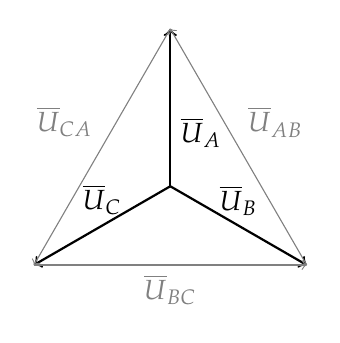
\begin{tikzpicture}
  \draw (0,0) coordinate (N);
  \draw (90:2) coordinate (A);
  \draw (-30:2) coordinate (B);
  \draw (-150:2) coordinate (C);
  \draw[->, thick] (N) -- (A) node[below right, midway] {$\overline{U}_A$};
  \draw[->, thick] (N) -- (B) node[above, midway] {$\overline{U}_B$};
  \draw[->, thick] (N) -- (C) node[above, midway] {$\overline{U}_C$};
  \draw[->, color = gray] (B) -- (A) node[above right, midway] {$\overline{U}_{AB}$};
  \draw[->, color = gray] (C) -- (B) node[below, midway] {$\overline{U}_{BC}$};
  \draw[->, color = gray] (A) -- (C) node[above left, midway] {$\overline{U}_{CA}$};
\end{tikzpicture}
\end{document}